\documentclass[tikz,border=6pt]{standalone}

% общий стиль (подключается через TEXINPUTS)
% tikz-style.tex (общий стиль для всех TikZ-картинок)
\RequirePackage[T1,T2A]{fontenc}
\RequirePackage[utf8]{inputenc}

% Palatino-подобный шрифт (как в MathJax часто воспринимается «более вытянутым»)
\RequirePackage{txfonts}
% txfonts даёт предупреждение по кириллице (T2A/txr не определён).
% Оставляем txfonts для математики, а текстовый шрифт возвращаем на Computer Modern,
% чтобы не искать T2A/txr и убрать предупреждения.
\renewcommand{\rmdefault}{cmr}
\renewcommand{\sfdefault}{cmss}
\renewcommand{\ttdefault}{cmtt}

\RequirePackage{tikz}
\RequirePackage{xcolor}
\usetikzlibrary{calc}

% цвета
\definecolor{lightgreen}{RGB}{214,234,214}
\definecolor{darkgreen}{HTML}{0B7A0B}
\definecolor{darkred}{HTML}{DF0000}

\definecolor{midgreen}{HTML}{2E9B2E}
\definecolor{palegreen}{RGB}{235,246,235}
\definecolor{olivegreen}{HTML}{3E6B2F}

\definecolor{lightred}{RGB}{255,220,220}
\definecolor{midred}{HTML}{E04545}
\definecolor{darkred2}{HTML}{A80000}

\definecolor{lightblue}{RGB}{220,232,255}
\definecolor{midblue}{HTML}{2E5BD6}
\definecolor{darkblue}{HTML}{0B2E8A}

\definecolor{lightgray}{RGB}{240,240,240}
\definecolor{midgray}{RGB}{170,170,170}
\definecolor{darkgray}{RGB}{80,80,80}

\definecolor{vtxfill}{RGB}{86,193,255}
\definecolor{vennfill}{RGB}{220,232,255}


% единый набор стилей TikZ
\tikzset{
    lab/.style={
        font=\fontsize{24}{32}\selectfont
    }
}


\definecolor{vtxfill}{RGB}{86,193,255} % #56C1FF

\begin{document}
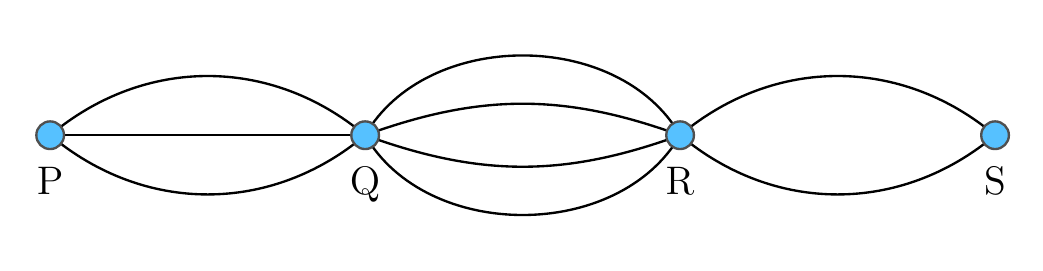
\begin{tikzpicture}[x=1cm,y=1cm, line cap=round, line join=round]

% vertex + edge styles (match the book template)
\tikzset{
  main/.style={draw=black, line width=0.85pt},
  vtx/.style={circle, draw=darkgray, fill=vtxfill, line width=0.85pt, minimum size=10pt, inner sep=0pt},
  vlab/.style={font=\Large},
}

  % nodes
  \coordinate (P) at (0,0);
  \coordinate (Q) at (4,0);
  \coordinate (R) at (8,0);
  \coordinate (S) at (12,0);

  % edges P--Q (top arc + straight + bottom arc)
  \draw[main] (P) to[out=40,in=140] (Q);
  \draw[main] (P) -- (Q);
  \draw[main] (P) to[out=-40,in=-140] (Q);

  % edges Q--R (four arcs, pulled toward center)
  \draw[main] (Q) to[out=60,in=120] (R);
  \draw[main] (Q) to[out=20,in=160] (R);
  \draw[main] (Q) to[out=-20,in=-160] (R);
  \draw[main] (Q) to[out=-60,in=-120] (R);

  % edges R--S (two arcs)
  \draw[main] (R) to[out=40,in=140] (S);
  \draw[main] (R) to[out=-40,in=-140] (S);

  % vertices
  \node[vtx] at (P) {};
  \node[vtx] at (Q) {};
  \node[vtx] at (R) {};
  \node[vtx] at (S) {};

  % labels
  \node[vlab, below=8pt] at (P) {P};
  \node[vlab, below=8pt] at (Q) {Q};
  \node[vlab, below=8pt] at (R) {R};
  \node[vlab, below=8pt] at (S) {S};

\end{tikzpicture}
\end{document}
